\section{Shear from Zernike coefficients} \label{sec:ell_zernike} 

We use Section 5.1 of \cite{jarvis_telescope_2008} to write down our aberration model, along with Section 10.3 of \cite{dodelson_modern_2003} to write down the ellipticity and shear in terms of PSF shape and size: 

\begin{equation}
d, a, c, s \xrightarrow{\text{\cite{jarvis_telescope_2008}}} Q(x, y), S(x, y) \xrightarrow{\text{\cite{dodelson_modern_2003}}} \gamma_1, \gamma_2
\end{equation}

Coefficients of the Zernike polynomials are field-of-view dependent and can be parameterized by position $x, y$ on the sky. We consider contributions from the first few dominant coefficients and define the following:
\begin{align}
d &= A_\text{defocus} \\
a &= A_\text{astigmation-c} + i A_\text{astigmation-s} \\
c &= A_\text{coma-c} + i A_\text{coma-s} \\
s &= A_\text{spherical}
\end{align}

The shape and size of the PSF are then given respectively as:
\begin{align}
Q(X, Y) &= \frac{\int dx dy I(x, y) (x+iy)^2}{\int dx dy I(x, y)} = 4 \Big(d+\frac{4}{3}s \Big) a + \frac{1}{3} c^2\\
S(X, Y) &= \frac{\int dx dy I(x, y) |x+iy|^2}{\int dx dy I(x, y)} = 2 \Big(d+\frac{4}{3}s \Big)^2 + 2 |a|^2 + \frac{2}{3} |c|^2 + \frac{4}{9} s^2\\
\end{align}
with the integral centered at $X, Y$. 

Ellipticity $\epsilon = \epsilon_1 + i \epsilon_2$ can be written as:
\begin{align}
\epsilon = \epsilon_1 + i \epsilon_2 &= \frac{q_{xx} - q_{yy}}{q_{xx} + q_{yy}} + i \frac{2 q_{xy}}{q_{xx} + q_{yy}}\\
&= \frac{1}{\int dx dy I(x, y) (x^2 + y^2)} \int dx dy I(x, y) \Big( x^2 + i^2 y^2 + 2ixy \Big) \\
&= Q \Big/ S
\end{align}

In the weak lensing limit, 
\begin{align}
\gamma_1 = \Re(Q / S) \Big/ 2 && \gamma_2 = \Im(Q / S) \Big/ 2
\end{align}

\newpage
\section{Toy Models} \label{sec:toy_models}

\subsection{Constant coefficients (large field-of-view)}

\begin{align}
\Delta \alpha \times \Delta \delta &= 8 \degree \times 8 \degree \\
n_\star &= 8 \times 8 \times 100 \\
d &= 10^{-1} \\
s &= 10^{-2} \\
a &= 10^{-2} + i \times 3 \times 10^{-3} \\
c &= 10^{-2} + i \times 3 \times 10^{-3}
\end{align}

\begin{figure}[h]
\centering
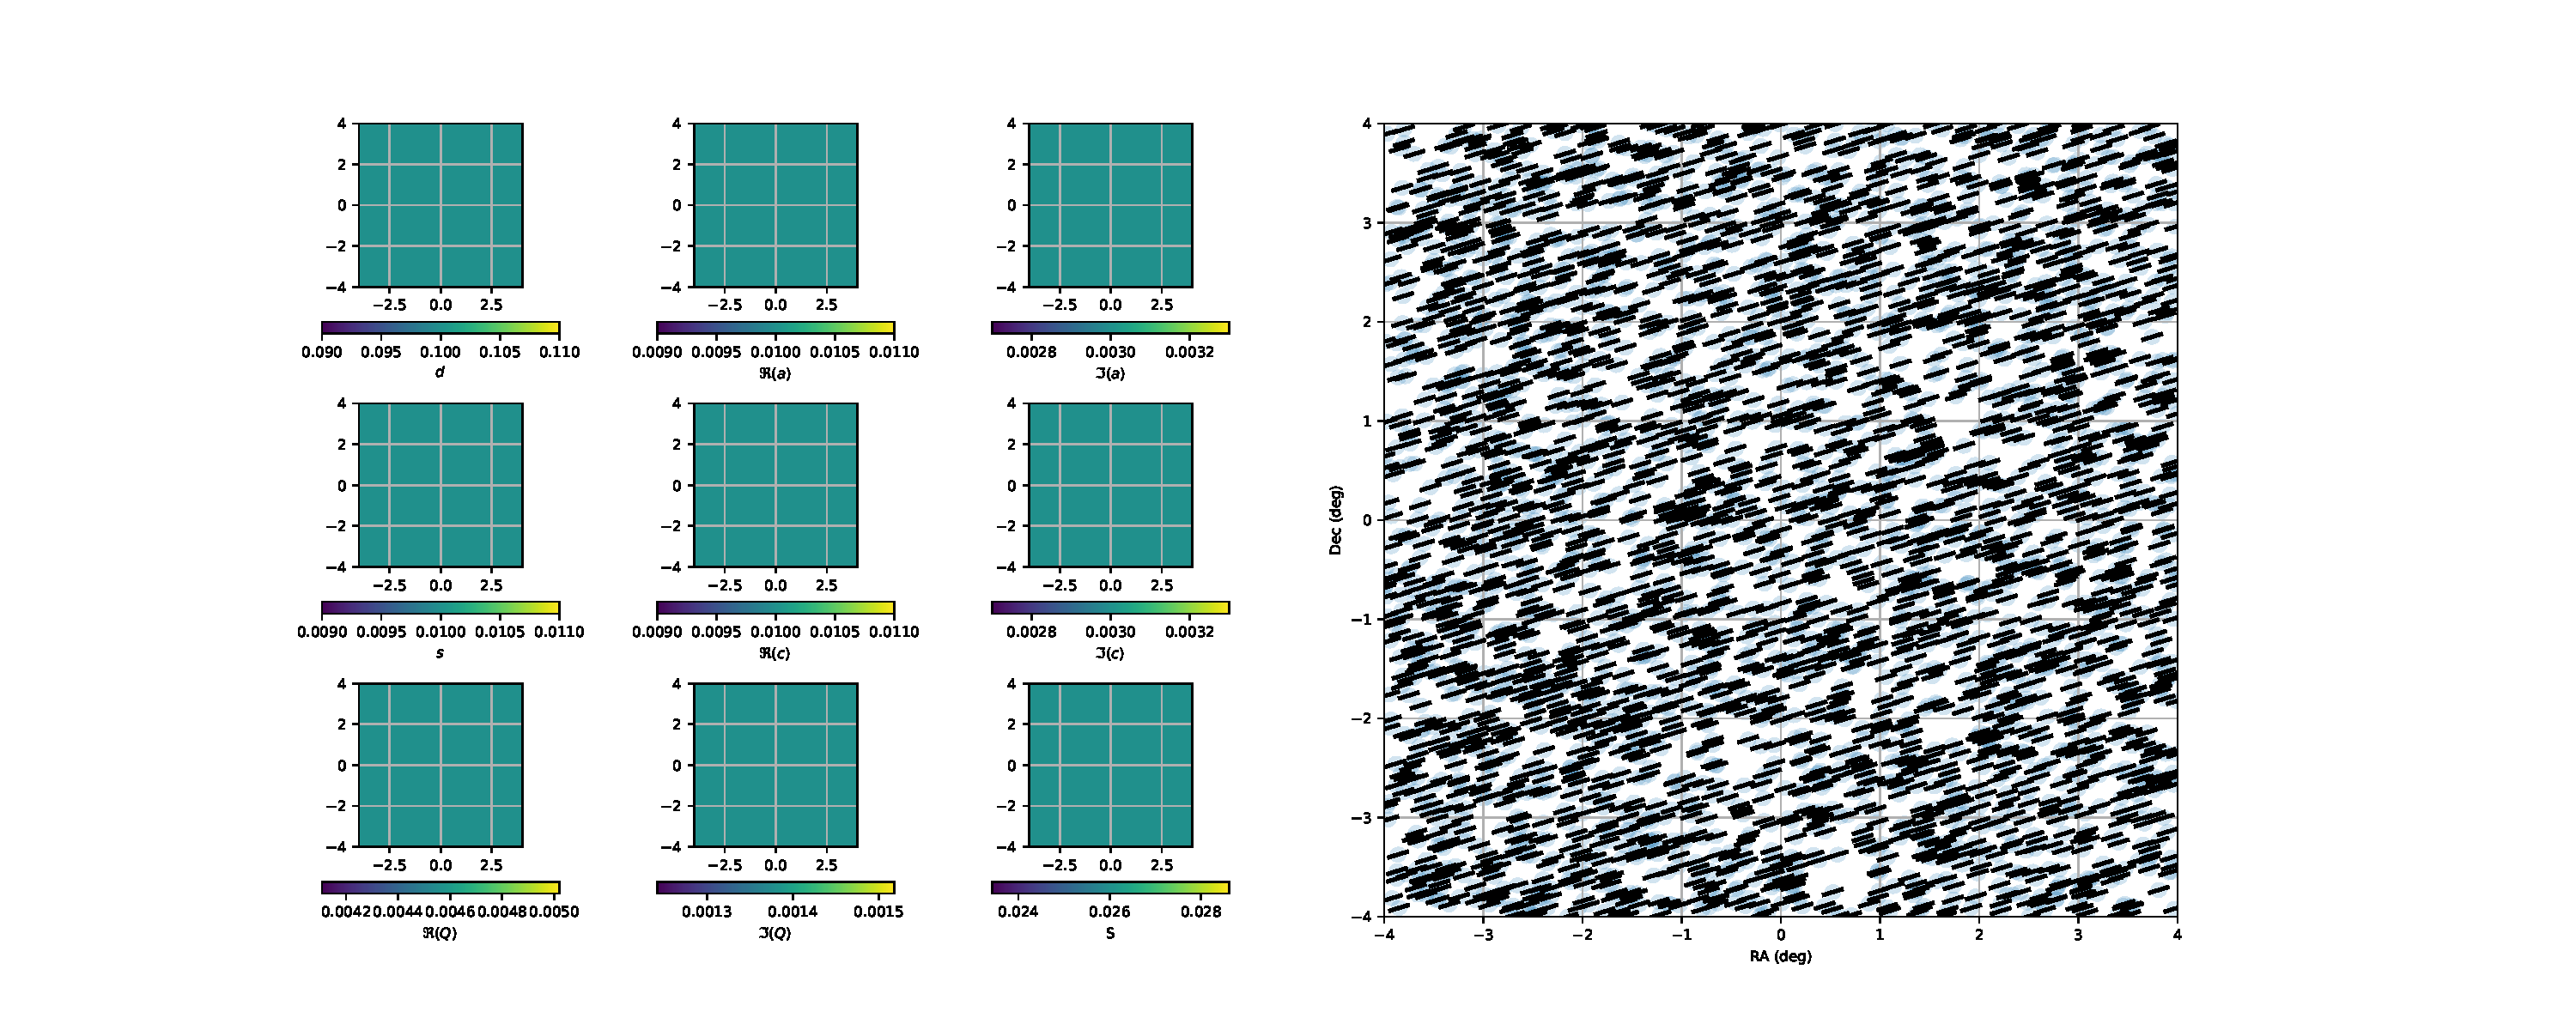
\includegraphics[width=\textwidth]{figs/20230109_constant/coeff_shear.pdf}
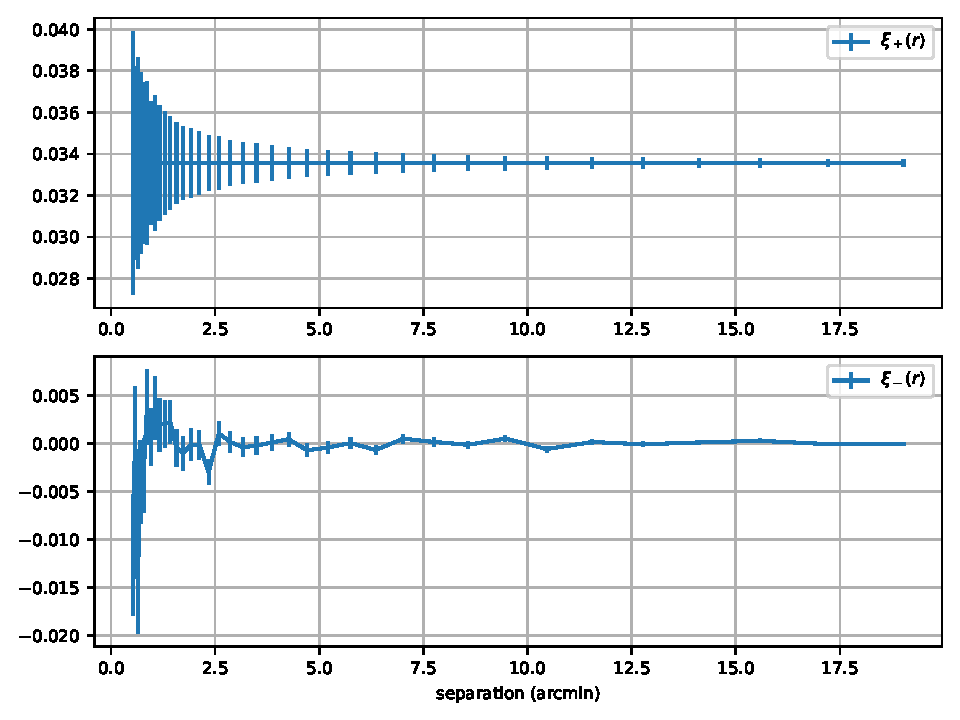
\includegraphics[width=0.48\textwidth]{figs/20230109_constant/2point.pdf}
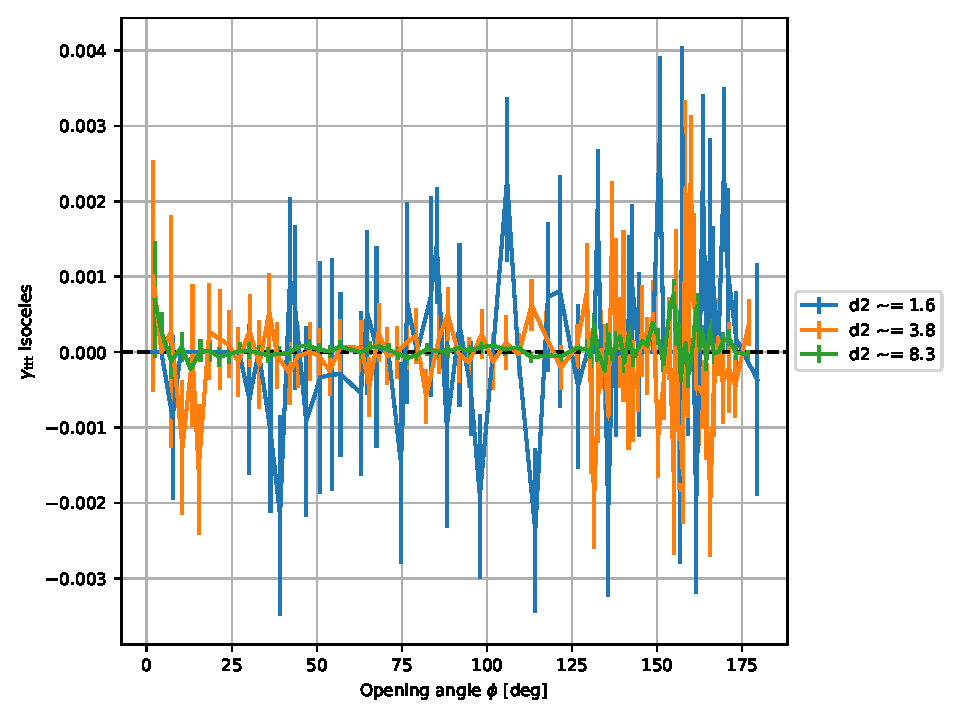
\includegraphics[width=0.48\textwidth]{figs/20230109_constant/3point.pdf}
\caption{Constant coefficients.}
\label{fig:constant}
\end{figure}

\newpage
\subsection{Radial dependence on imaginary parts (large field-of-view)}

\begin{align}
\Delta \alpha \times \Delta \delta &= 8 \degree \times 8 \degree \\
n_\star &= 8 \times 8 \times 100 \\
d &= 10^{-1} \\
s &= 10^{-2} \\
a &= 10^{-2} + i \times 3 \times 10^{-3} (x^2+y^2) \\
c &= 10^{-2} + i \times 3 \times 10^{-3} (x^2+y^2)
\end{align}

\begin{figure}[h]
\centering
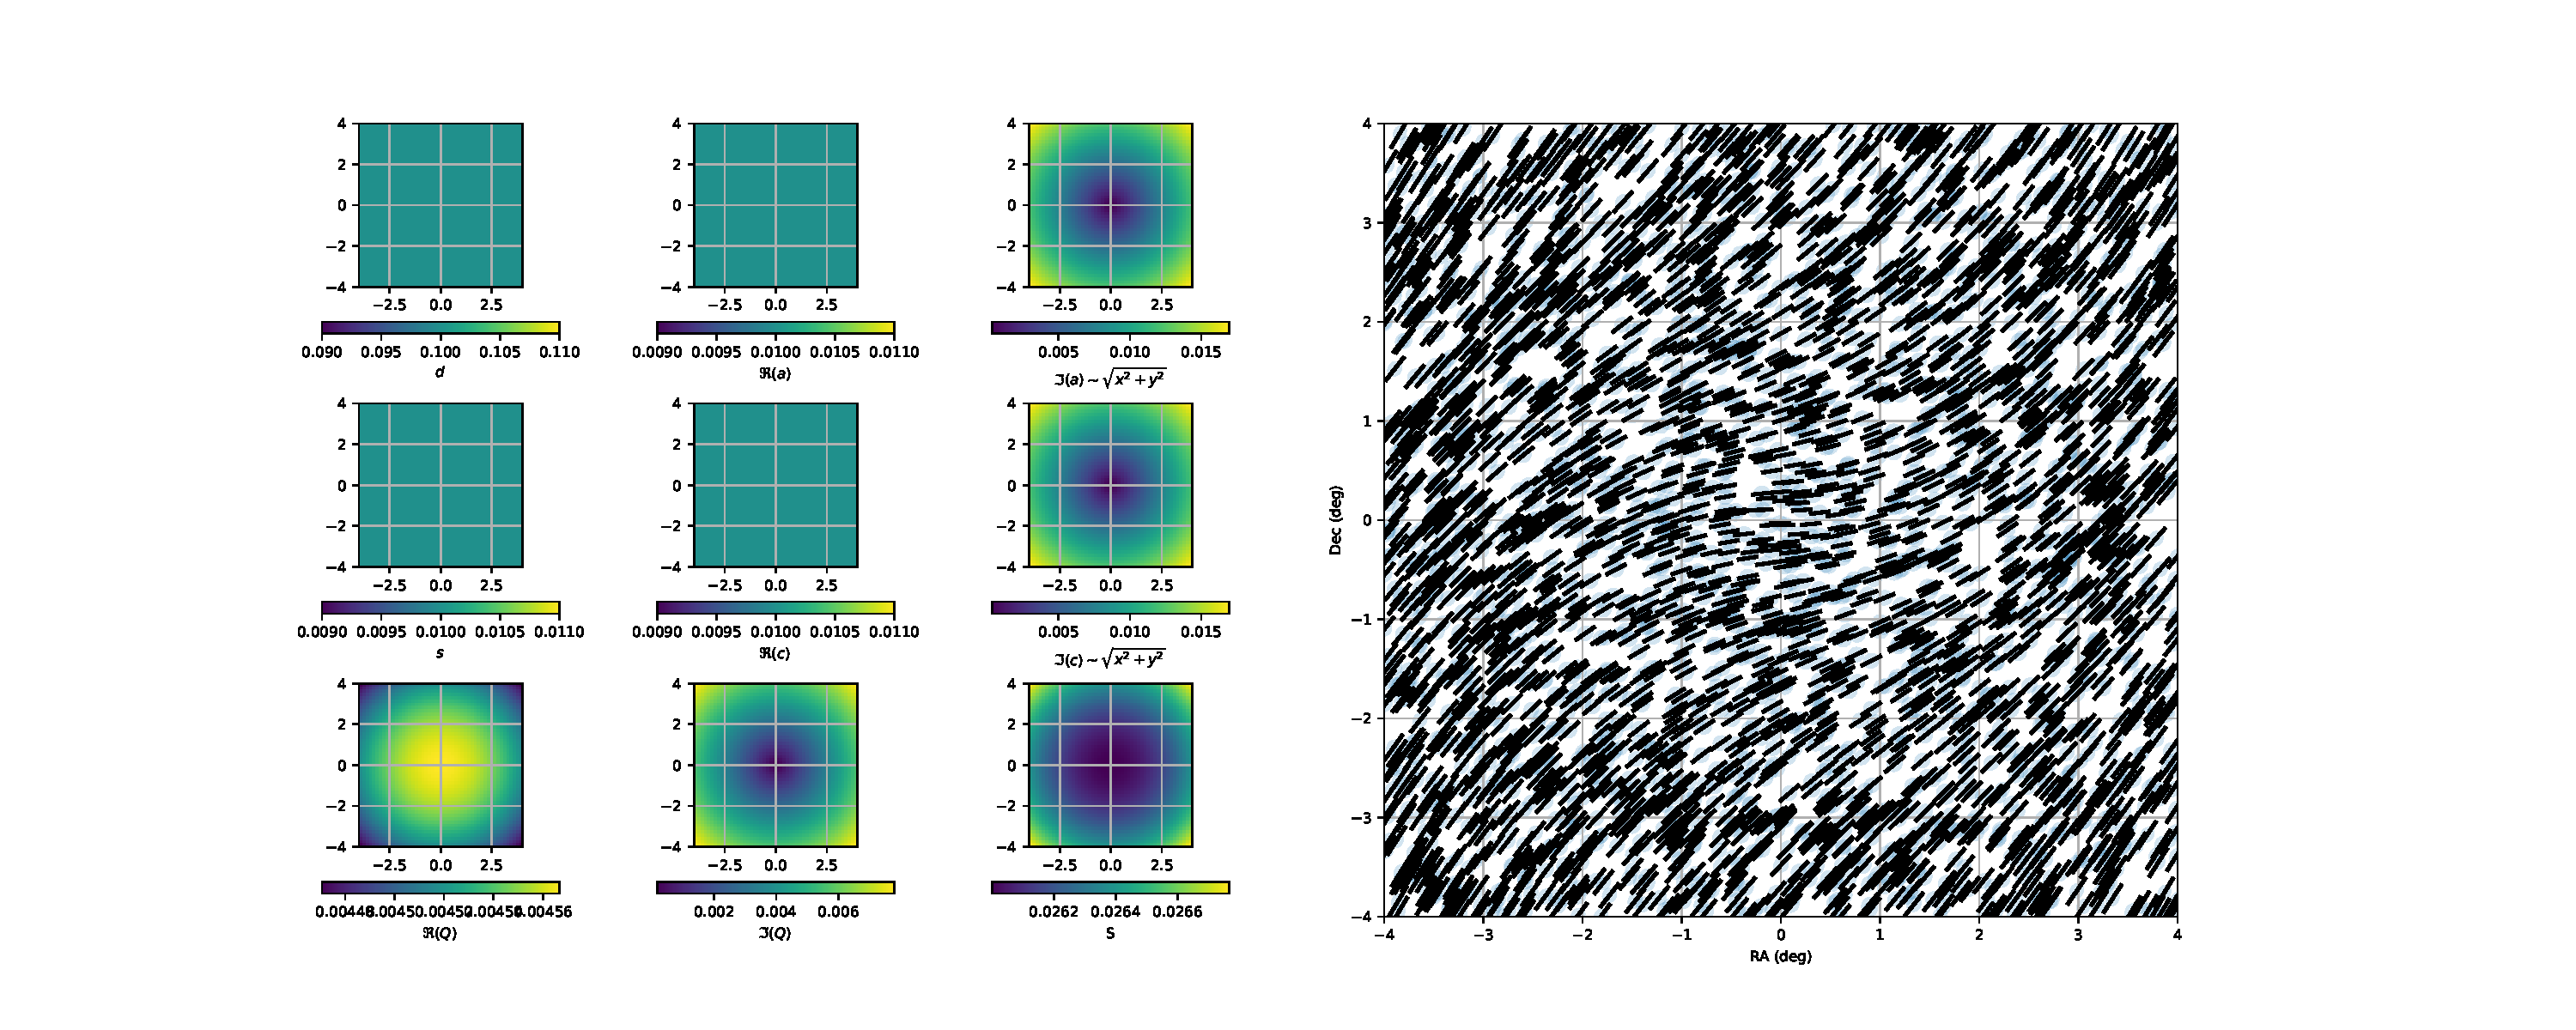
\includegraphics[width=\textwidth]{figs/20230109_radial_imag/coeff_shear.pdf}
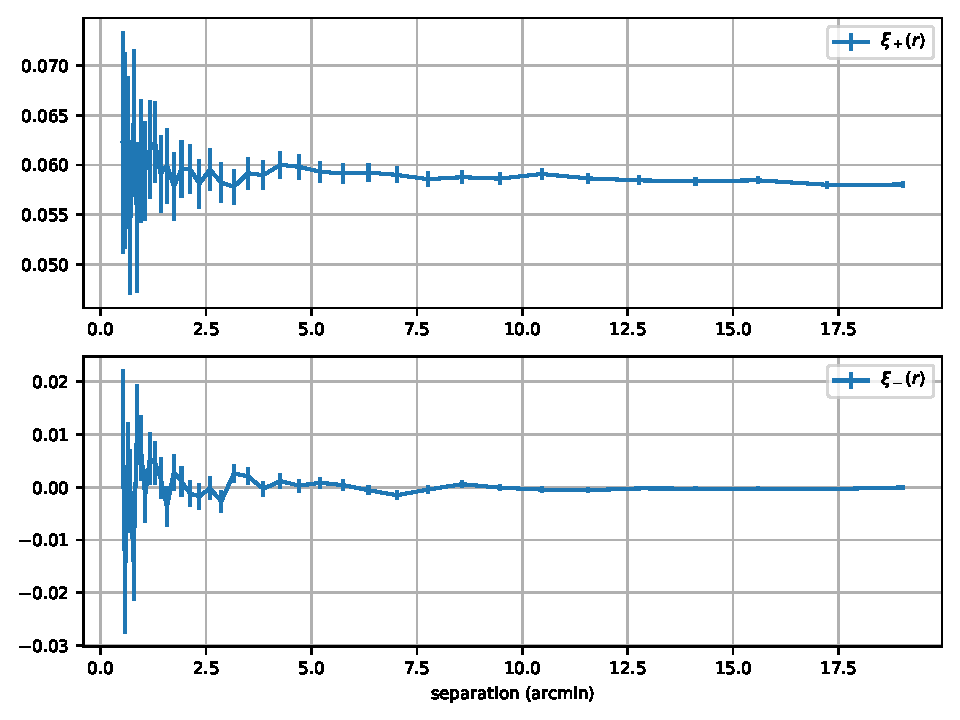
\includegraphics[width=0.48\textwidth]{figs/20230109_radial_imag/2point.pdf}
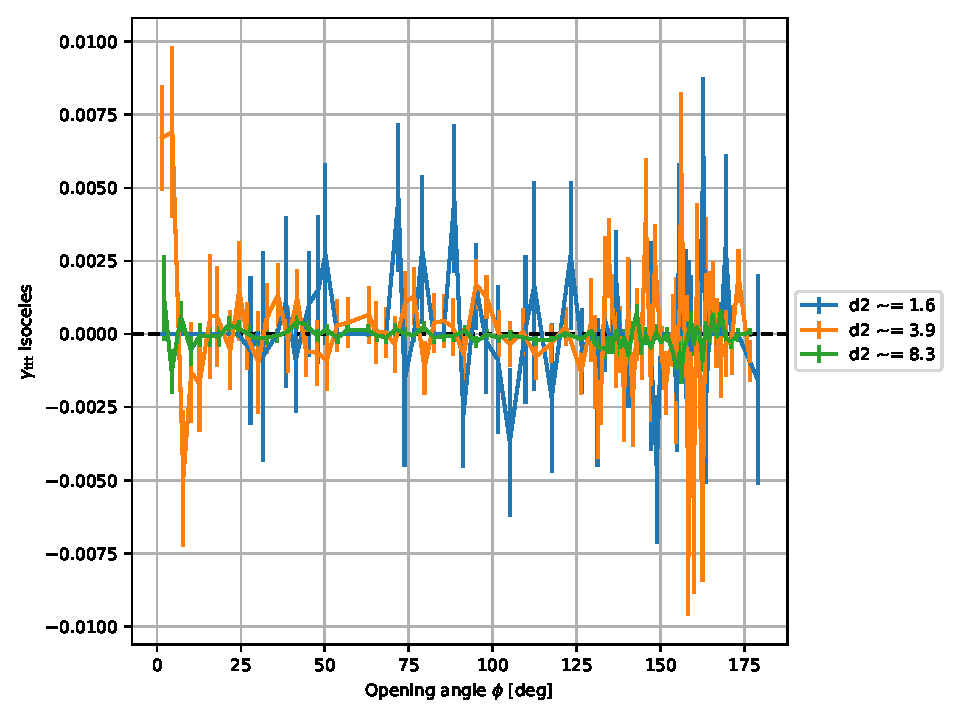
\includegraphics[width=0.48\textwidth]{figs/20230109_radial_imag/3point.pdf}
\caption{Radial coefficients.}
\label{fig:radial}
\end{figure}

\newpage
\subsection{Constant coefficients (regular field-of-view, high number density)}

\begin{align}
\Delta \alpha \times \Delta \delta &= 1.2 \degree \times 1.2 \degree \\
n_\star &= 1.2 \times 1.2 \times 10^4 \\
d &= 10^{-1} \\
s &= 10^{-2} \\
a &= 10^{-2} + i \times 3 \times 10^{-3} \\
c &= 10^{-2} + i \times 3 \times 10^{-3}
\end{align}

\begin{figure}[h]
\centering
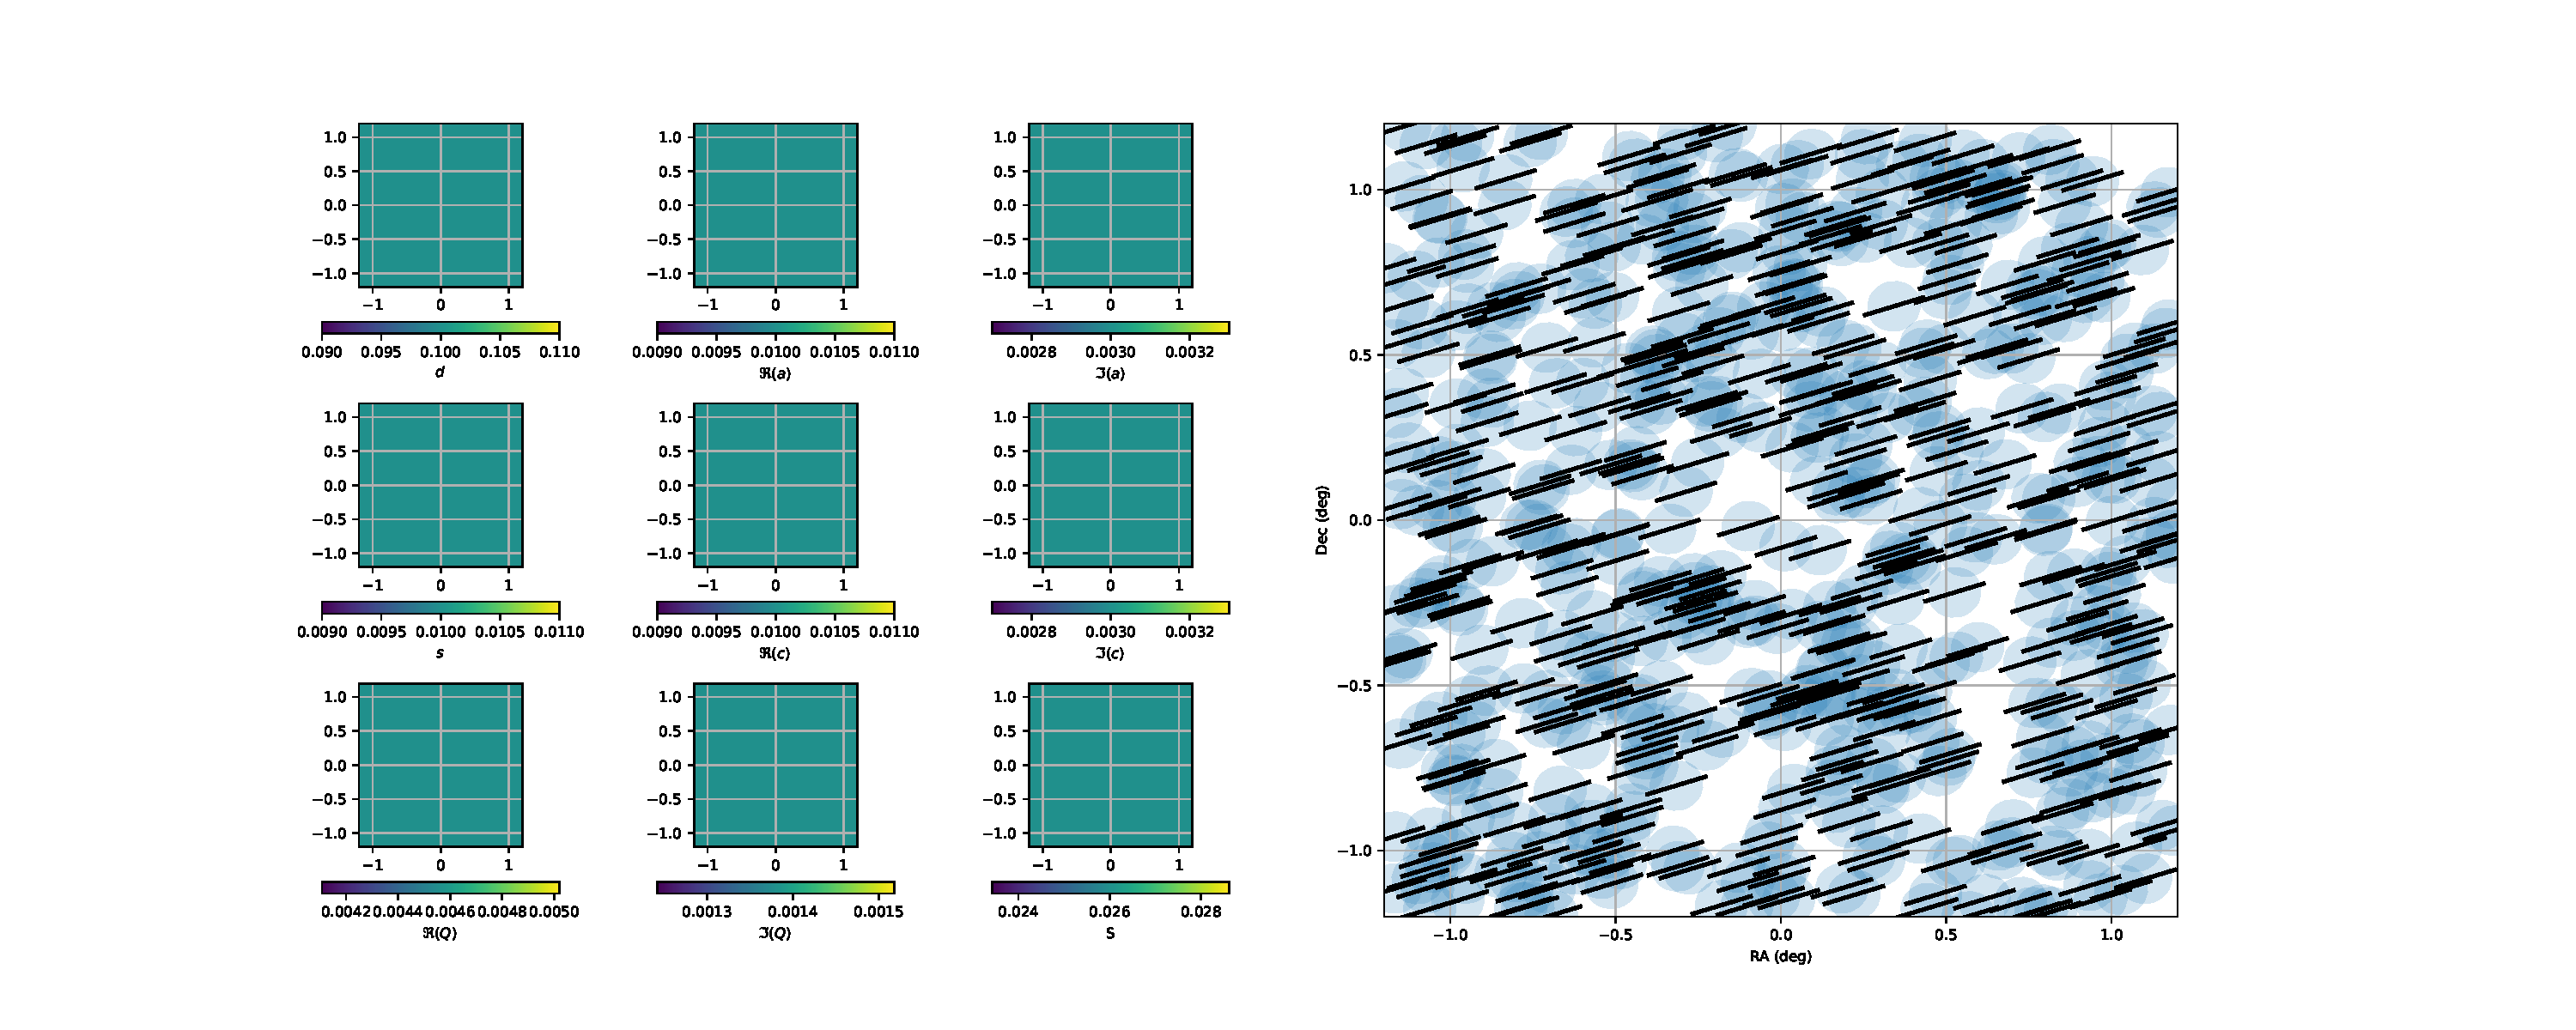
\includegraphics[width=\textwidth]{figs/20230110_constant/coeff_shear.pdf}
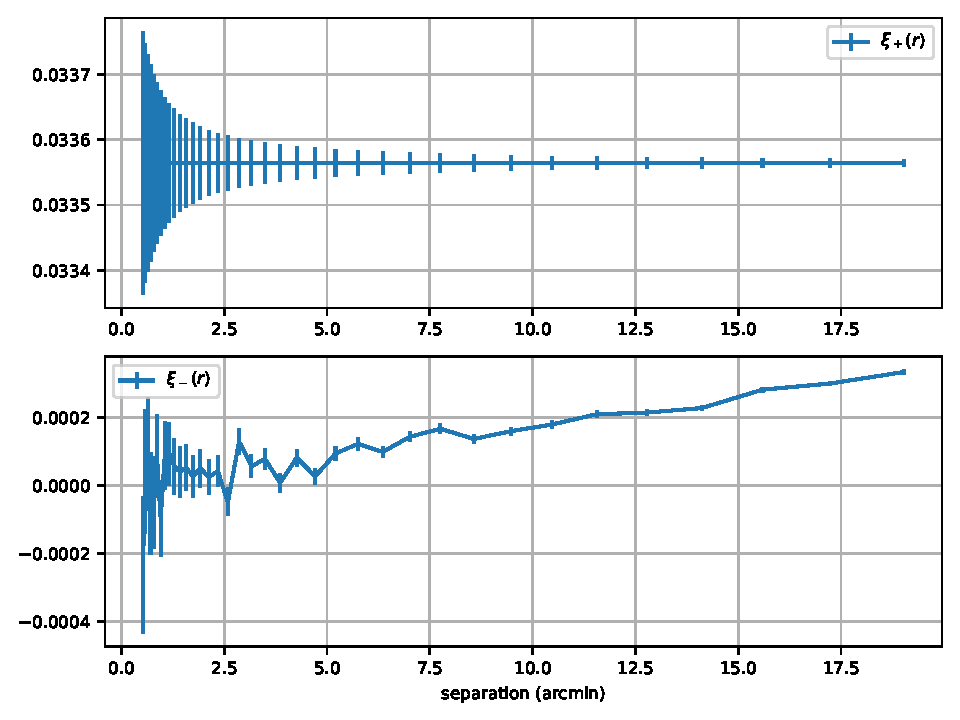
\includegraphics[width=0.48\textwidth]{figs/20230110_constant/2point.pdf}
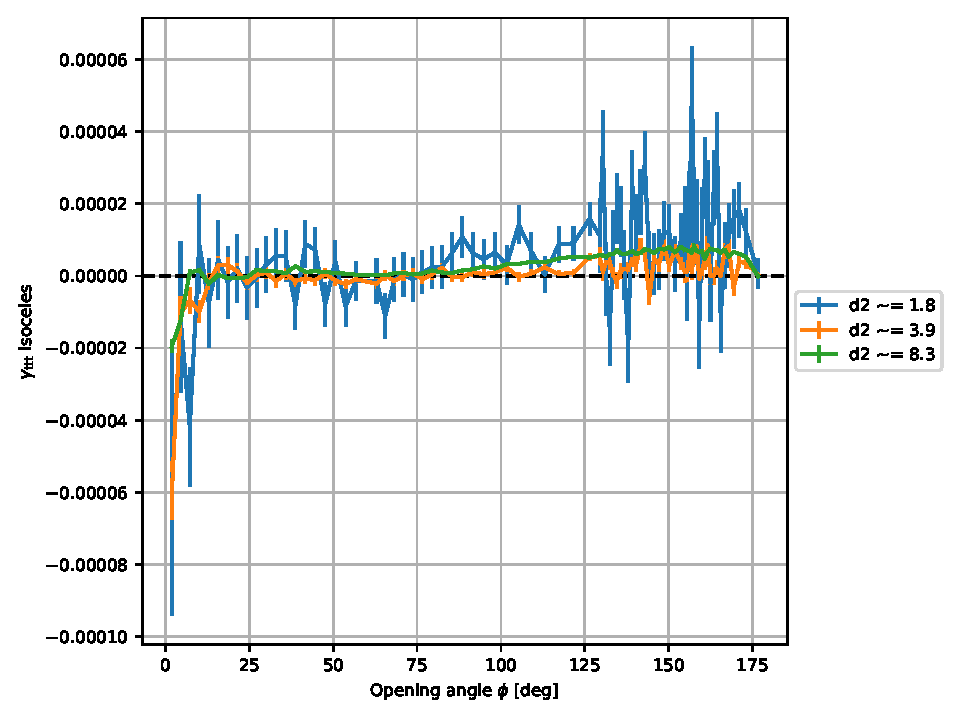
\includegraphics[width=0.48\textwidth]{figs/20230110_constant/3point.pdf}
\caption{Constant coefficients. PSF number thinned by factor of 100.}
\label{fig:constant}
\end{figure}

\newpage
\subsection{Radial dependence on imaginary parts (regular field-of-view, high number density)}

\begin{align}
\Delta \alpha \times \Delta \delta &= 1.2 \degree \times 1.2 \degree \\
n_\star &= 1.2 \times 1.2 \times 10^4 \\
d &= 10^{-1} \\
s &= 10^{-2} \\
a &= 10^{-2} + i \times 3 \times 10^{-3} (x^2+y^2) \\
c &= 10^{-2} + i \times 3 \times 10^{-3} (x^2+y^2)
\end{align}

\begin{figure}[h]
\centering
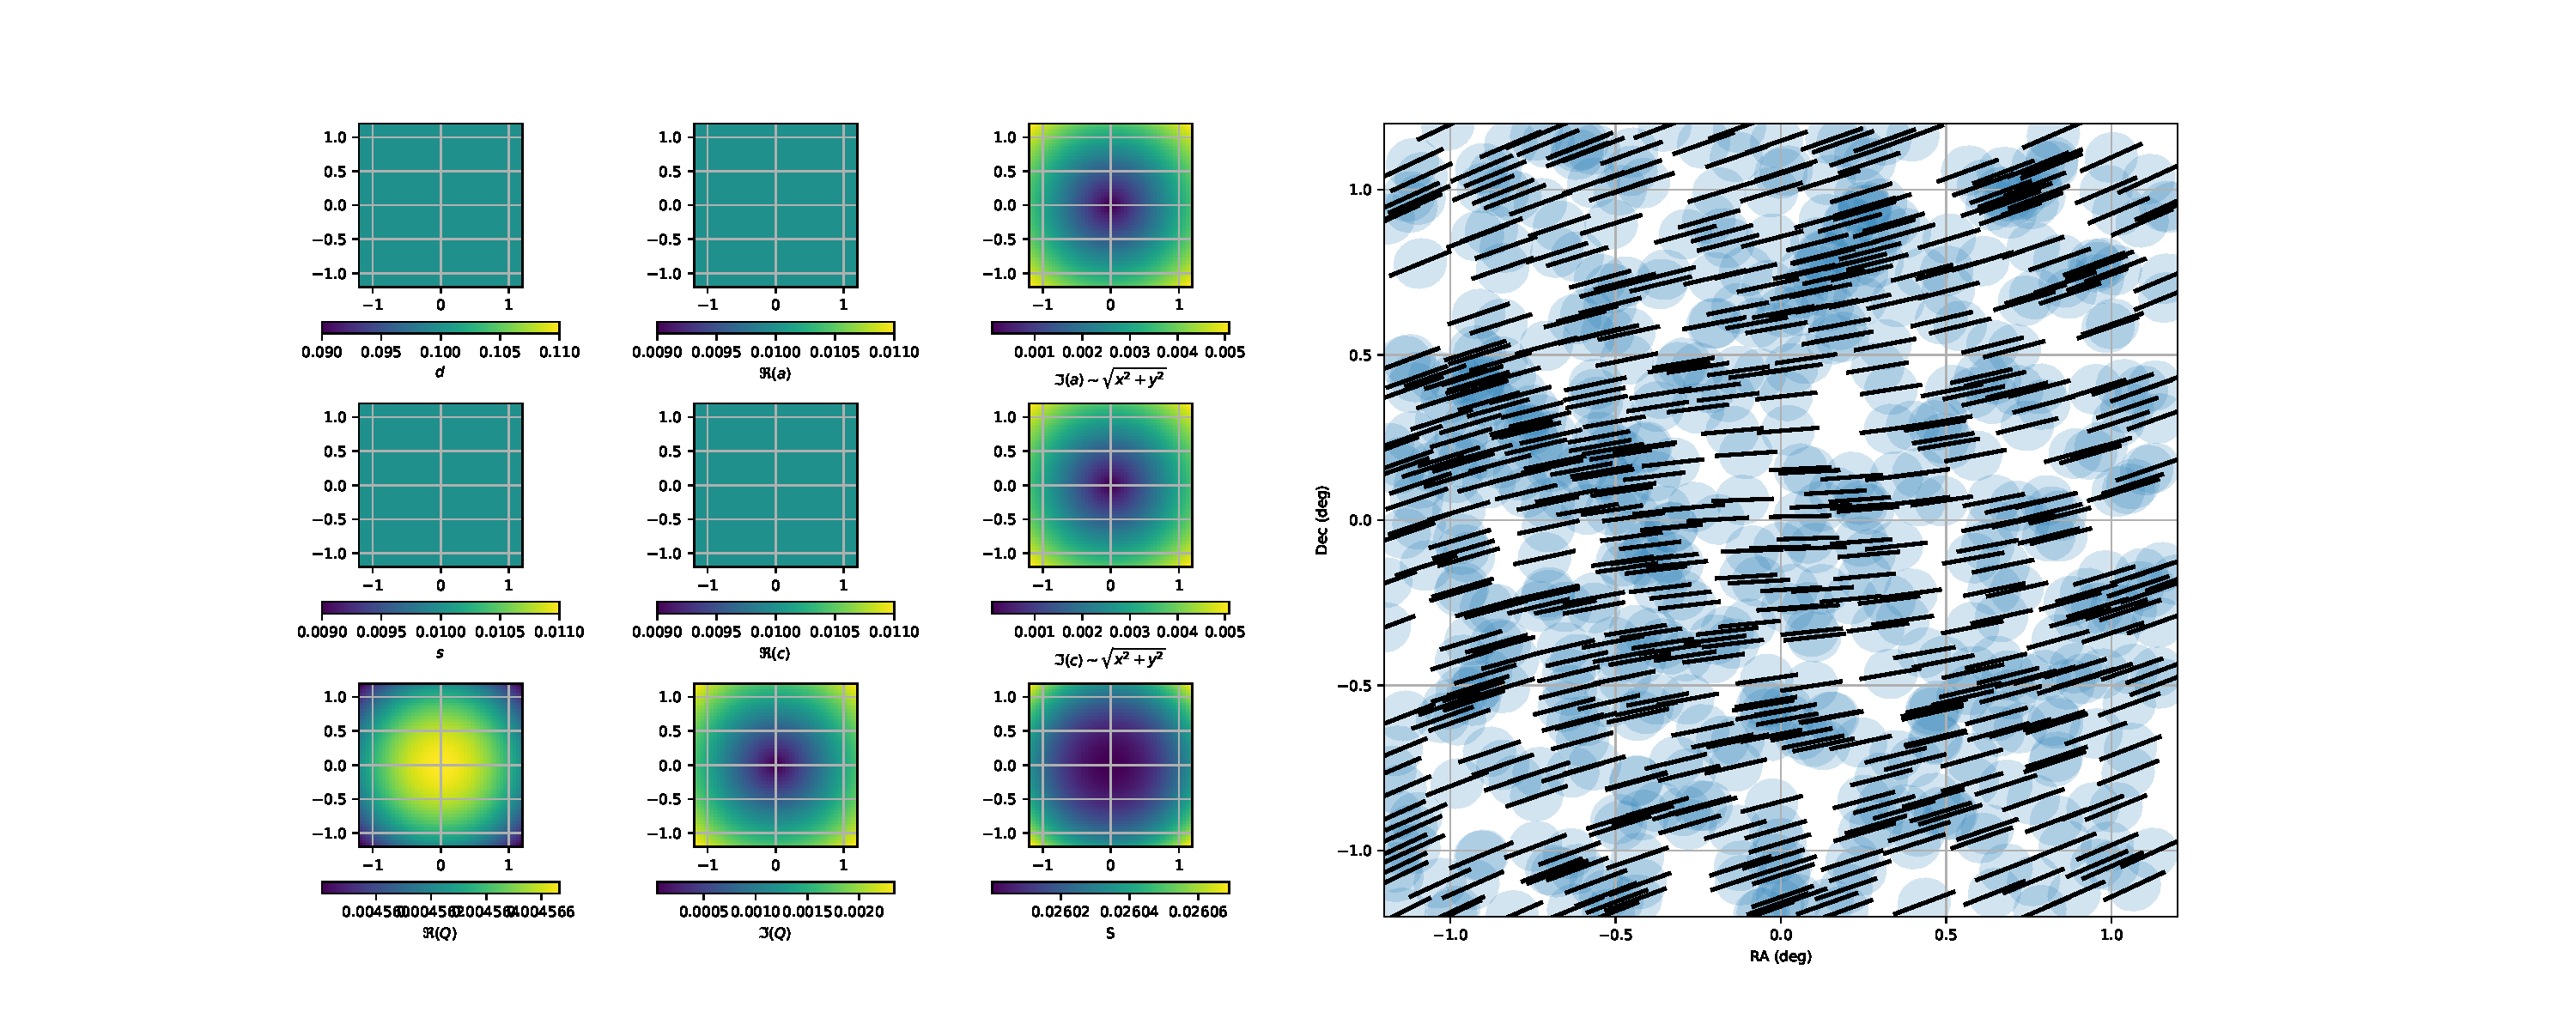
\includegraphics[width=\textwidth]{figs/20230110_radial_imag/coeff_shear.pdf}
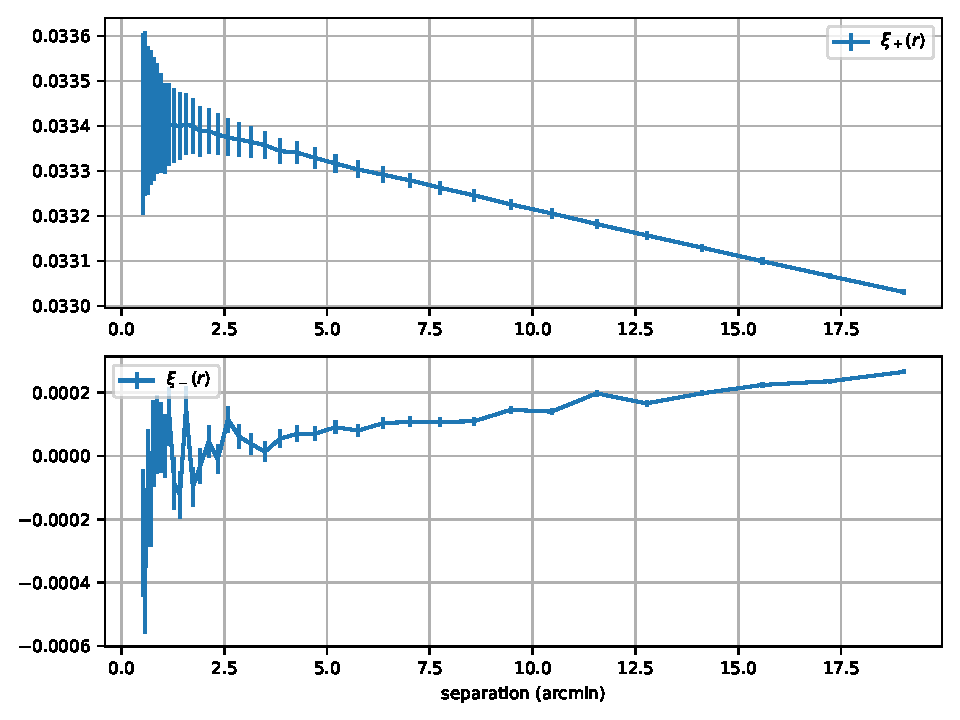
\includegraphics[width=0.48\textwidth]{figs/20230110_radial_imag/2point.pdf}
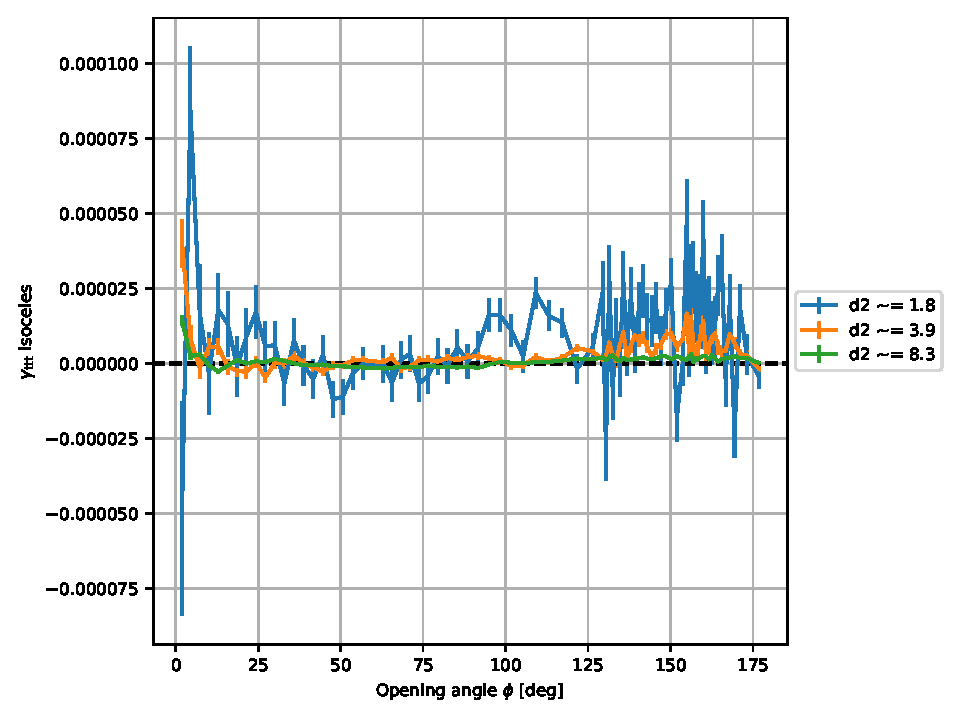
\includegraphics[width=0.48\textwidth]{figs/20230110_radial_imag/3point.pdf}
\caption{Radial coefficients. PSF number thinned by factor of 100.}
\label{fig:radial}
\end{figure}

\newpage
\subsection{Model from \cite{jarvis_telescope_2008}}

\begin{align}
\Delta \alpha \times \Delta \delta &= 1.2 \degree \times 1.2 \degree = R\times R \\
n_\star &= 1.2 \times 1.2 \times 10^5 \\
d &= -0.006 + \Re{\big( (0.009 - 0.003i) \times (x - i y) / R \big)} \\
s &= 0 \\
a &= 0.014 - 0.011 i + (0.001 - 0.002 i) * (x + i y) / R \\
c &= -0.039 + i \times -0.010
\end{align}

\begin{figure}[h]
\centering
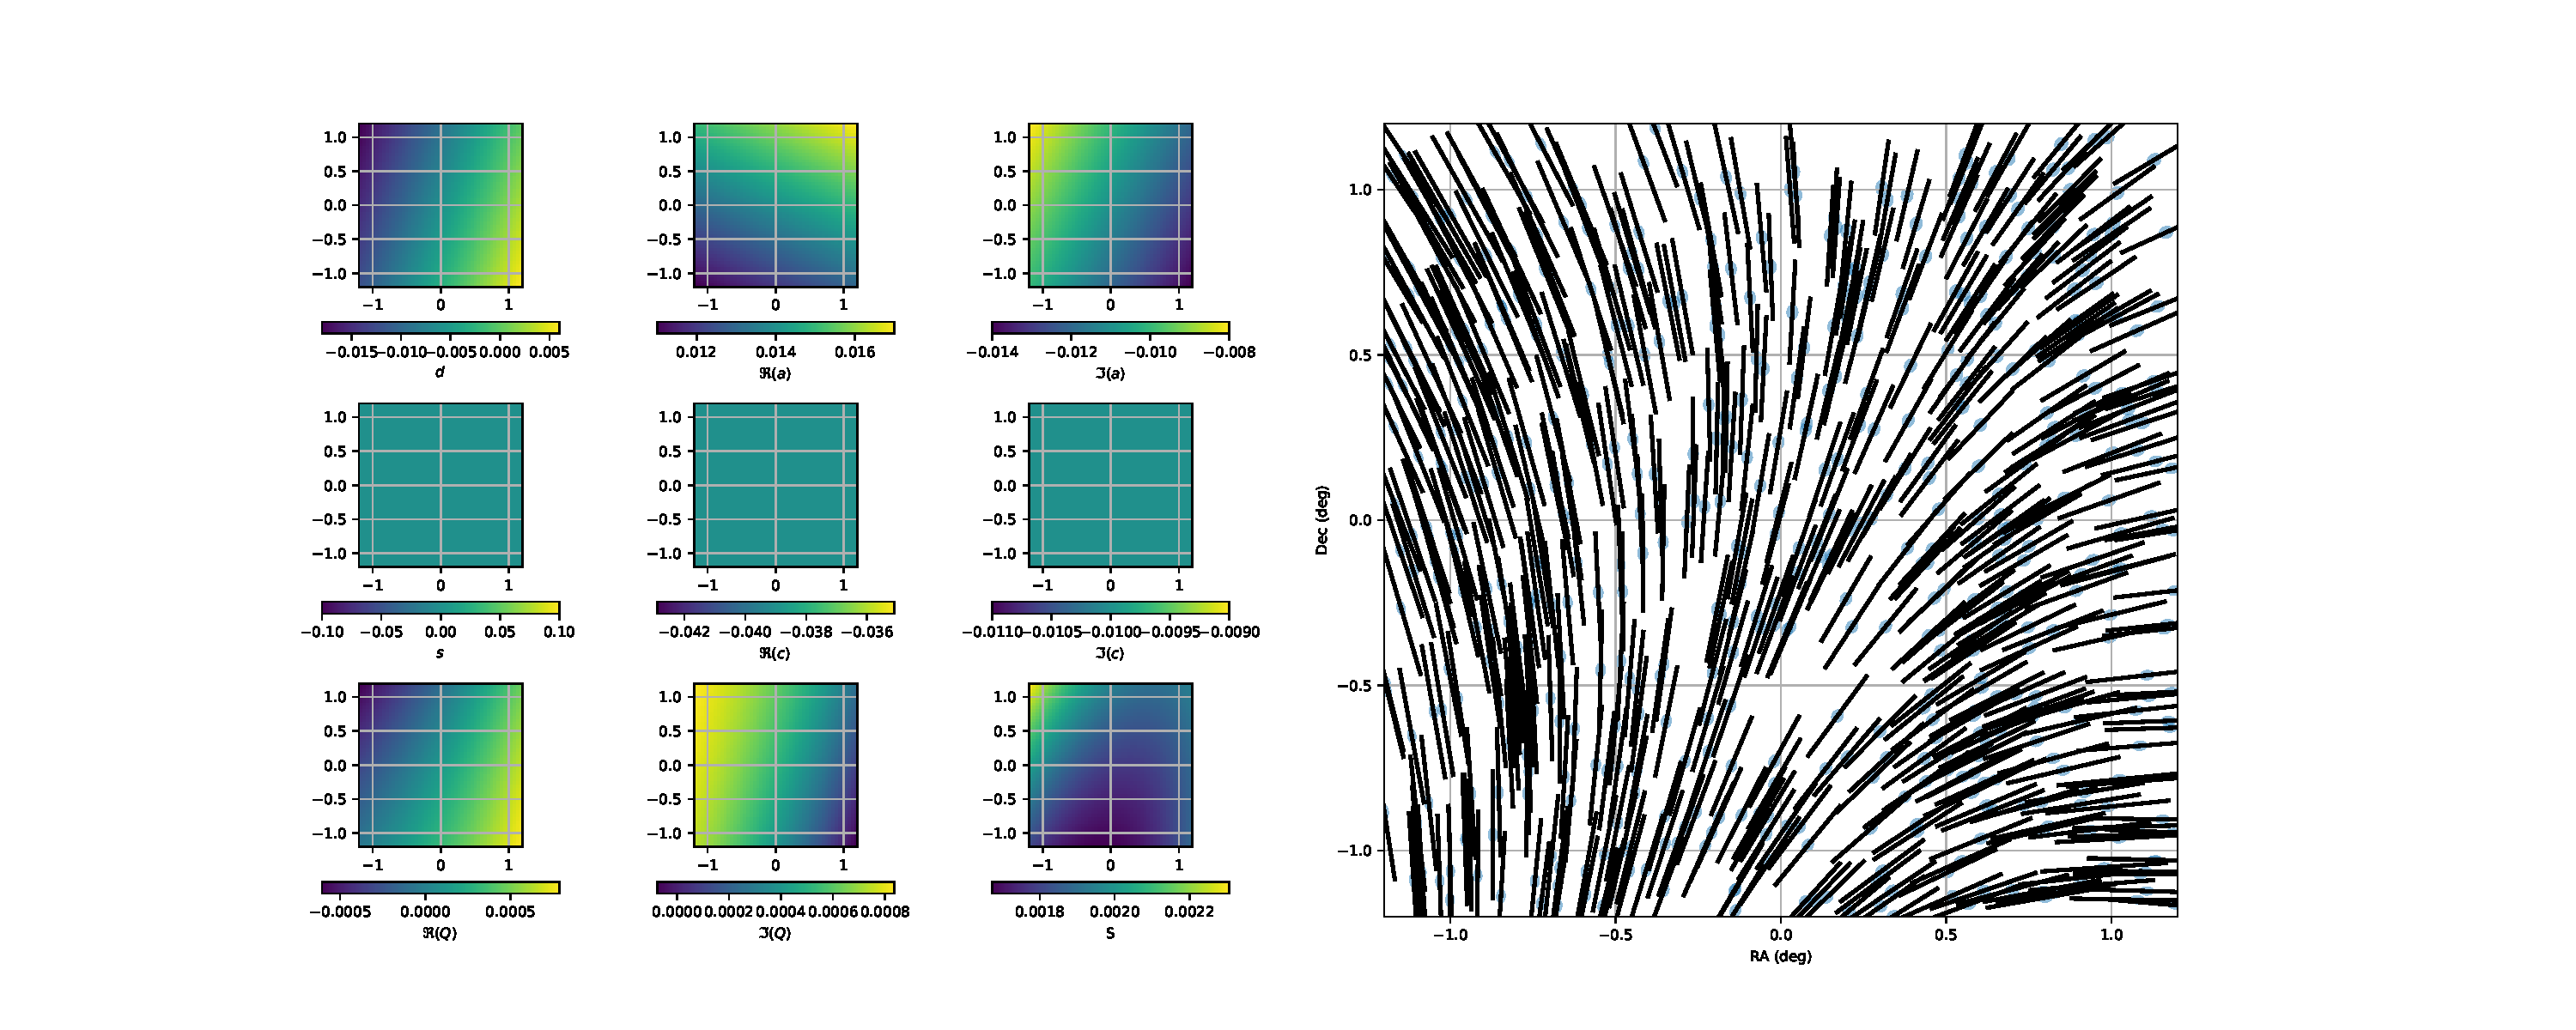
\includegraphics[width=\textwidth]{figs/20230111_mike_paper/coeff_shear.pdf}
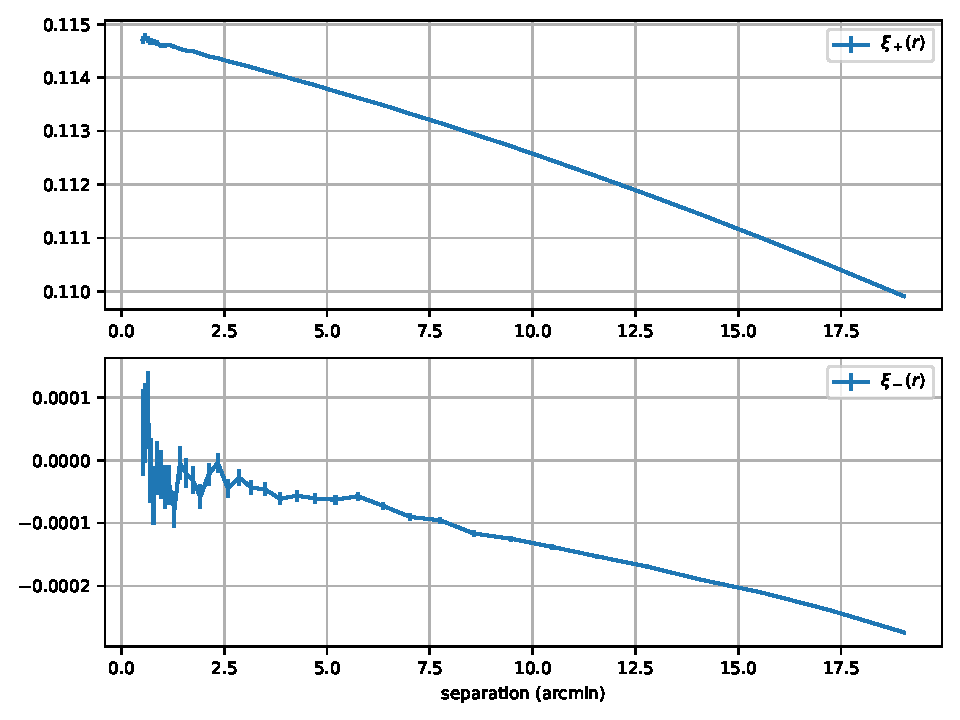
\includegraphics[width=0.48\textwidth]{figs/20230111_mike_paper/2point.pdf}
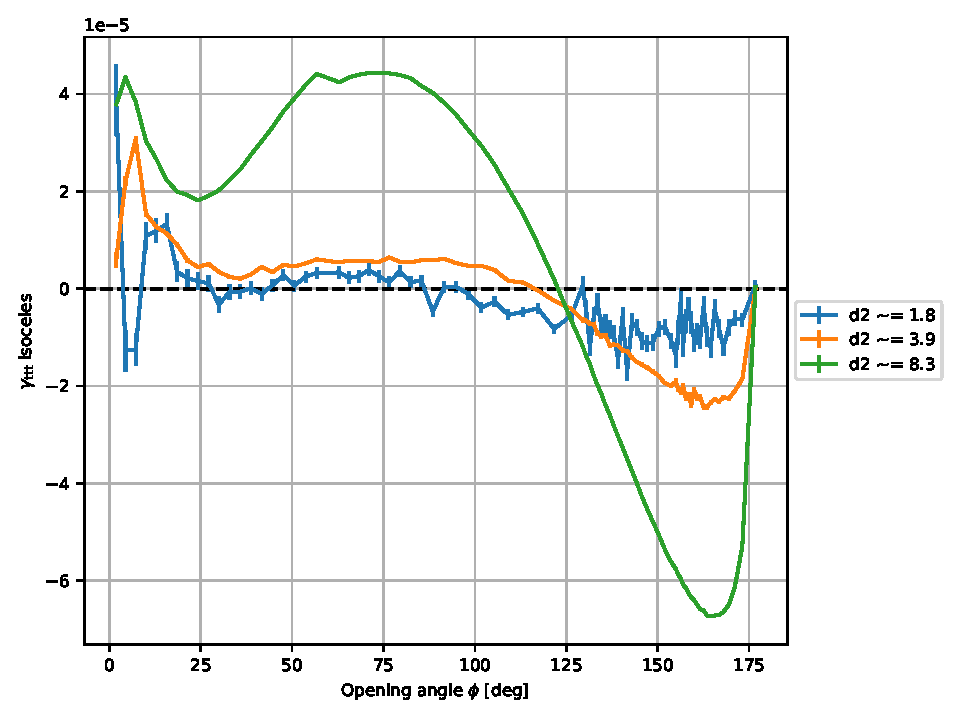
\includegraphics[width=0.48\textwidth]{figs/20230111_mike_paper/3point.pdf}
\caption{\cite{jarvis_telescope_2008} model. PSF number thinned by factor of 1000.}
\label{fig:radial}
\end{figure}
